\documentclass{article}
\usepackage[utf8]{inputenc}
\usepackage{amsmath}
\usepackage{amssymb}
\usepackage{amsthm}
\usepackage{tikz}
\setlength{\parindent}{0pt}

\newtheorem*{theorem}{Theorem}
\newtheorem*{definition}{Definition}
\newtheorem*{lemma}{Lemma}
\newtheorem*{corollary}{Corollary}
\newtheorem{example}{Example}
\newtheorem*{trick}{Trick}
\newtheorem*{question}{Question}

\title{Lecture 14: Non-independent Variables}
\author{}
\date{}

\begin{document}
    
\maketitle

\section{Motivation}

We often need to deal with multivariable functions with non-independent 
variables. A real world example is that in physics some physical quantities can 
be described as a function of pressure $P$, volume $V$, and temperature $T$, 
where these three quantities satisfy a relation as $PV = nRT$.

In general, a multivariable function with non-independent variables can be 
described as $f(x, y, z)$, where $g(x, y, z) = c$.

In the previous lecture, we use Lagrange multipliers to find the local maximum 
or minimum points for such functions. We want to study more details about those 
functions, such as calculating the rate of change of the function value with 
respect to a certain variable.

\section{Partial Derivatives of Non-independent Variables}

Since $g(x, y, z) = c$, any of the three variables can be described as a 
function of other two variables, though in most cases it is hard to find the 
explicit formula for the function. For example, we know that the variable $z$ 
can be described as $z = z(x, y)$. In this case, $x$ and $y$ are considered as 
independent variables. Though we might not be able to explicitly express the 
non-independent variables as functions of independent variables, we still want 
to study the relationship, such as how those non-independent variables change 
with regards to independent variables.

\begin{example}
  For $x^2 + yz + z^3 = 8$ at $(2, 3, 1)$, calculate the partial derivatives of 
  $z$ with regards to $x$ and $y$.

  According to the total differential formula,
  \begin{equation*}
    2xdx + zdy + (y + 3z^2)dz = 0
  \end{equation*}
  At the point $(2, 3, 1)$, the total differential becomes
  \begin{equation*}
    4dx + dy + 6dz = 0
  \end{equation*}
  If we consider $z$ as the non-independent variable, in other words 
  $z = z(x, y)$, then
  \begin{equation*}
    dz = -\frac{1}{6}(4dx + dy)
  \end{equation*}
  By total differential formula, we can derive that
  \begin{gather*}
    \frac{\partial z}{\partial x} = -\frac{2}{3} \\
    \frac{\partial z}{\partial y} = -\frac{1}{6} \\
  \end{gather*}
  The above partial derivatives can also be derived by setting $x$ and $y$ as 
  constant respectively, hence the $dx$ and $dy$ would become 0 respectively in 
  the total differential formula of $z$.
\end{example}

In general, when $g(x, y, z) = c$, according to the total differential formula,
\begin{gather*}
  dg = g_xdx + g_ydy + g_zdz = 0 \\
  dz = -\frac{g_x}{g_z}dx - \frac{g_y}{g_z}dy \\
  \frac{\partial z}{\partial x} = -\frac{g_x}{g_z} \\
  \frac{\partial z}{\partial y} = -\frac{g_y}{g_z} \\
\end{gather*}
Using the same method, we can also find $\frac{\partial x}{\partial y}$, 
$\frac{\partial x}{\partial z}$, $\frac{\partial y}{\partial x}$, 
$\frac{\partial y}{\partial z}$ in the cases where they are considered as the 
non-independent variables.

\section{Pitfall in Notation}

\begin{example}
  Suppose that there is a multivariable function $f(x, y) = x + y$, then
  \begin{equation*}
    \frac{\partial f}{\partial x} = 1
  \end{equation*}
  With changes of variables $x = u$, and $y = u + v$, the function becomes
  \begin{equation*}
    f(u, v) = 2u + v
  \end{equation*}
  Then
  \begin{equation*}
    \frac{\partial f}{\partial u} = 2
  \end{equation*}
  It turns out that although $x = u$,
  \begin{equation*}
    \frac{\partial f}{\partial x} \neq \frac{\partial f}{\partial u}
  \end{equation*}
  How to explain this?

  The reason is that the original notation of partial derivatives has implicit 
  meanings. In this case, $\frac{\partial f}{\partial x}$ means the rate of 
  change of $f$ with regards to $x$ while keeping $y$ constant, and 
  $\frac{\partial f}{\partial u}$ means the rate of change of $f$ with regards 
  to $u$ while keeping $v$ constant. While $x$ and $u$ are the same variables, 
  keeping $y$ constant and keeping $v$ constant are different. According to 
  $y = u + v$, when we vary $u$ or $x$, keeping $y$ constant means $v$ are going 
  to change as well, and keeping $v$ constant means $y$ are going to change.
\end{example}

Therefore, we need a new notation to make the implicit meaning of partial 
derivatives explicit:
\begin{gather*}
  (\frac{\partial f}{\partial x})_y: \textnormal{the rate of change of f with regards to x while keeping y constant} \\
  (\frac{\partial f}{\partial u})_v: \textnormal{the rate of change of f with regards to u while keeping v constant} \\
  (\frac{\partial f}{\partial x})_v: \textnormal{the rate of change of f with regards to x while keeping v constant} \\
\end{gather*}
Therefore, in terms of the above cases, the inequality relation actually 
describes:
\begin{equation*}
  (\frac{\partial f}{\partial x})_y \neq (\frac{\partial f}{\partial u})_v
\end{equation*}

The use case of the new notation in this lecture is that it helps us to specify 
among the variables of a multivariable function which ones are considered as 
independent. The variables appearing in the new notation are independent 
variables.

\section{Partial Derivatives of Function Value with regards to Independent Variables}

\begin{example}
  Find the rate of change of the area of the following triangle with regards to 
  the angle $\theta$ in the diagram.

  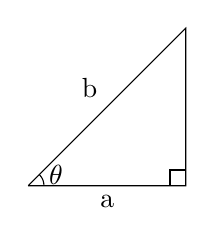
\begin{tikzpicture}
    [help line/.style={dashed}]
    \draw (0, 0) -- (2, 0) -- (2, 2) -- (0, 0);
    \draw (1, 0) node[below] {a};
    \draw (1, 1) node[above left] {b};
    \draw (0.2, 0) arc [start angle=0, end angle=45, radius=0.2] node[right] 
      {$\theta$};
    \draw (2, 0.2) -- (1.8, 0.2) -- (1.8, 0);
  \end{tikzpicture}

  Since the triangle is a right triangle, the three variables $a$, $b$, and 
  $\theta$ cannot be independent at the same time. They satisfy the following 
  constraint:
  \[ a = b\cos\theta \]
  According to the geometric knowledge, the area of the triangle is
  \[ A = \frac{1}{2}ab\sin\theta \]
  We need to find the rate of change of $A$ with regards to $\theta$.

  Since there is a non-independent variable, we need to discuss different 
  possible cases by considering which variables are considered as independent:
  \begin{itemize}
    \item If we consider the variables $a$ and $\theta$ as independent 
      variables, then the rate of change of $A$ with regards to $\theta$ can be 
      expressed as $(\frac{\partial A}{\partial \theta})_a$.
    \item If we consider the variables $b$ and $\theta$ as independent
      variables, then the rate of change of $A$ with regards to $\theta$ can be 
      expressed as $(\frac{\partial A}{\partial \theta})_b$.
  \end{itemize}

  Suppose we consider $a$ and $\theta$ as independent variables and want to find 
  $(\frac{\partial A}{\partial \theta})_a$, there are two methods:
  \begin{itemize}
    \item Method 1: Use the total differential formula.

      Let's look at the constraint first.
      \begin{gather*}
        a = b\cos\theta \\
        a - b\cos\theta = 0 \\
        da - \cos\theta db + b\sin\theta d\theta = 0 \\
        (\frac{\partial b}{\partial \theta})_a = b\tan\theta \\
      \end{gather*}
      Then we look at the multivariable function.
      \begin{gather*}
        A = \frac{1}{2}ab\sin\theta \\
        dA = \frac{1}{2}b\sin\theta da + \frac{1}{2}a\sin\theta db + \frac{1}{2}ab\cos\theta d\theta \\
      \end{gather*}
      When we try to calculate $(\frac{\partial A}{\partial \theta})_a$, we 
      consider the variable $a$ as constant. Then
      \begin{gather*}
        \frac{1}{2}b\sin\theta da = \frac{1}{2}b\sin\theta \cdot 0 = 0 \\
        \begin{split}
          \frac{1}{2}a\sin\theta db &= \frac{1}{2}a\sin\theta ((\frac{\partial b}{\partial \theta})_a d\theta + (\frac{\partial b}{\partial a})_\theta da) \\
                                    &= \frac{1}{2}a\sin\theta ((\frac{\partial b}{\partial \theta})_a d\theta + (\frac{\partial b}{\partial a})_\theta \cdot 0) \\
                                    &= \frac{1}{2}a\sin\theta \cdot (\frac{\partial b}{\partial \theta})_a \cdot d\theta \\
                                    &= \frac{1}{2}ab\sin\theta \tan\theta \cdot d\theta
        \end{split} \\
        \begin{split}
          dA &= \frac{1}{2}b\sin\theta da + \frac{1}{2}a\sin\theta db + \frac{1}{2}ab\cos\theta d\theta \\
             &= \frac{1}{2}ab\sin\theta \tan\theta \cdot d\theta + \frac{1}{2}ab\cos\theta d\theta \\
             &= \frac{1}{2}ab(\sin\theta \tan\theta + \cos\theta) d\theta \\
             &= \frac{1}{2}ab\sec\theta d\theta \\
        \end{split} \\
        (\frac{\partial A}{\partial \theta})_a = \frac{1}{2}ab\sec\theta \\
      \end{gather*}
    \item Method 2: Use the chain rule.
    
      According to the chain rule,
      \begin{gather*}
        (\frac{\partial A}{\partial \theta})_a = A_\theta (\frac{\partial \theta}{\partial \theta})_a + A_a (\frac{\partial a}{\partial \theta})_a + A_b (\frac{\partial b}{\partial \theta})_a \\
        (\frac{\partial A}{\partial \theta})_a = A_\theta \cdot 1 + A_a \cdot 0 + A_b (\frac{\partial b}{\partial \theta})_a \\
        (\frac{\partial A}{\partial \theta})_a = A_\theta + A_b (\frac{\partial b}{\partial \theta})_a \\
        (\frac{\partial A}{\partial \theta})_a = \frac{1}{2}ab\cos\theta + \frac{1}{2}a\sin\theta \cdot b\tan\theta \\
        (\frac{\partial A}{\partial \theta})_a = \frac{1}{2}ab(\cos\theta + \sin\theta \tan\theta) \\
        (\frac{\partial A}{\partial \theta})_a = \frac{1}{2}ab\sec\theta \\
      \end{gather*}
  \end{itemize}
  We can see the two methods reach to the same results.
\end{example}

\end{document}